\begin{figure}[htbp]
    \centering
    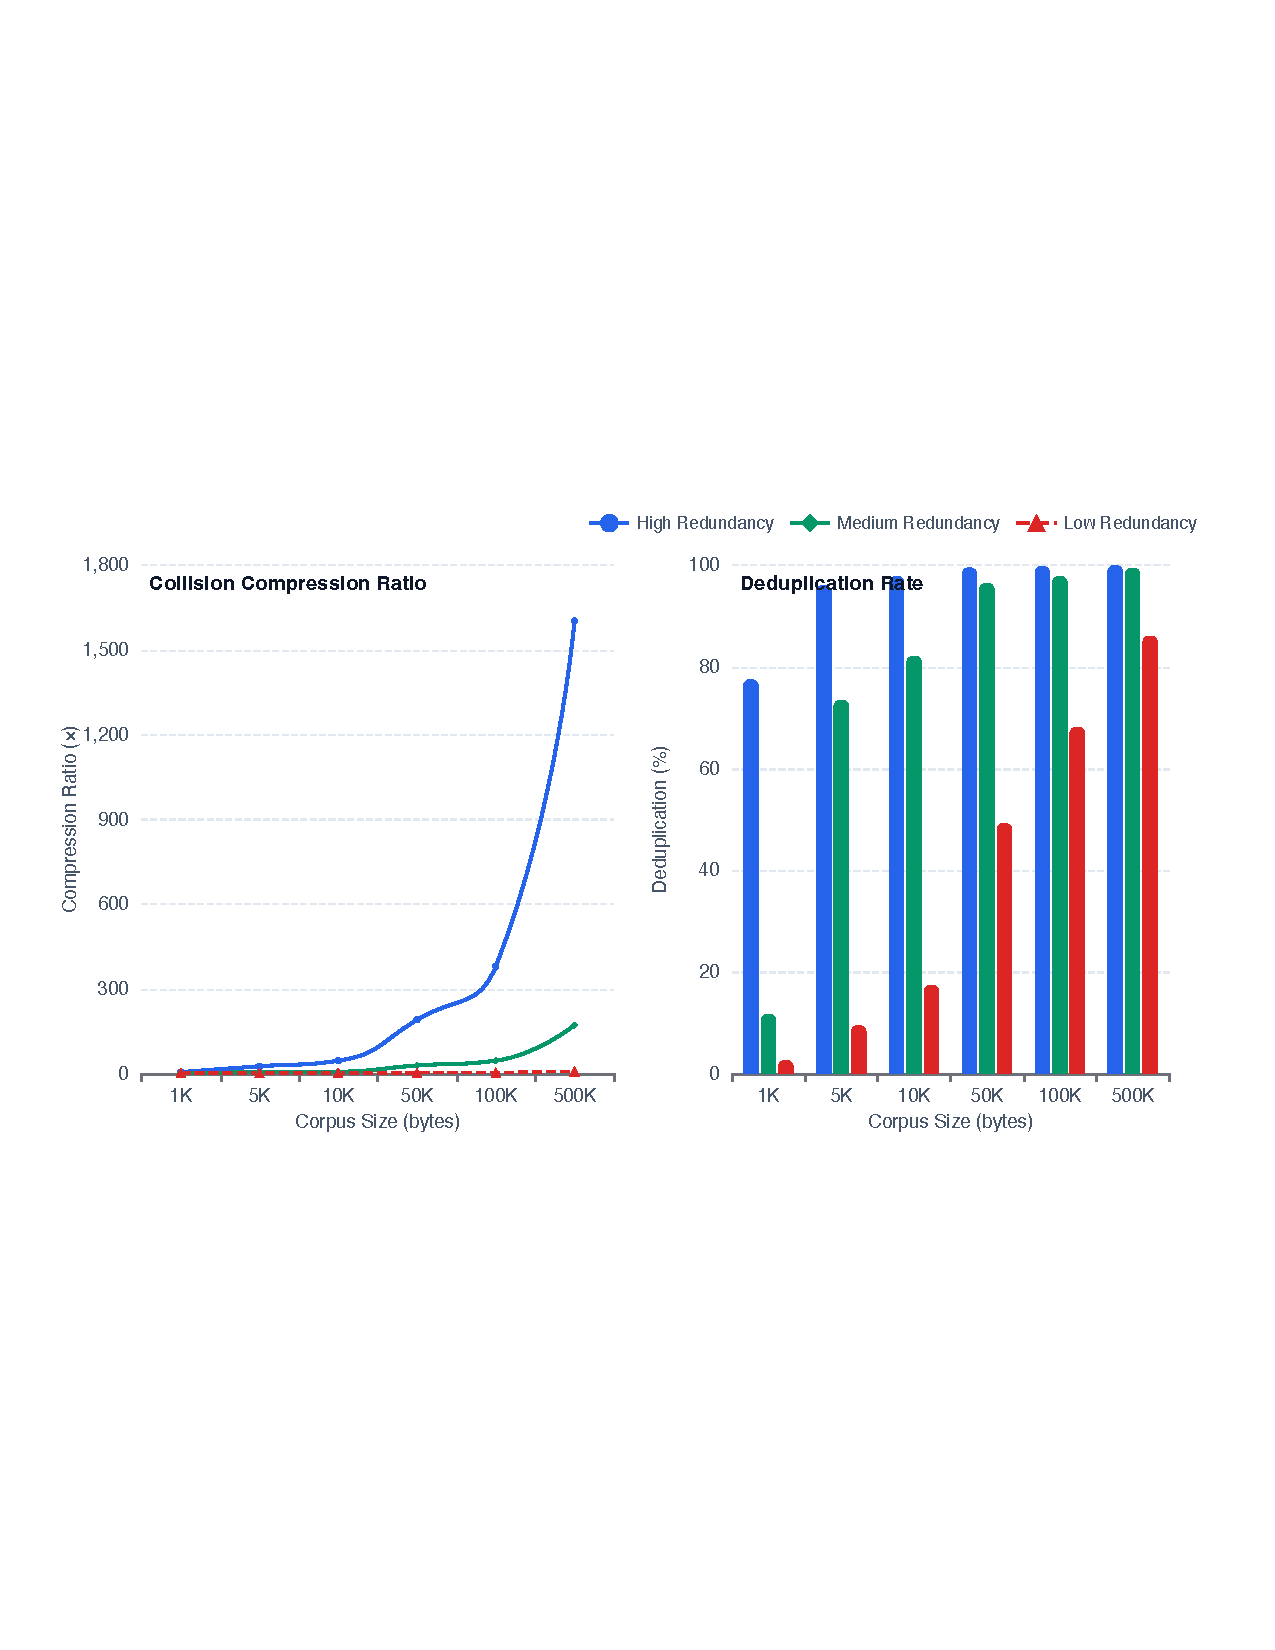
\includegraphics[width=1.0\textwidth]{compression_ratio.pdf}
    \caption{(Left) Compression ratio (raw tokens / unique index entries) vs corpus size across three redundancy profiles. High-redundancy data (repetitive sentences) achieves >100× compression as identical Morton keys collide and the LSM merge natively deduplicates. Low-redundancy data (pseudo-random bytes) converges to ~1× as expected from Shannon's limit. (Right) Deduplication rate: percentage of raw tokens eliminated by collision.}
    \label{fig:compression_ratio}
\end{figure}
